%%%%%%%%%%%%%%%%%%%%%%%%%%%%%%%%%%%%%%%%%%%%%%%%%%%%%%%%%%%%%%%%%%%%%%%%%%%%%%%%%%%%%%%%%%%%%%%
\section{Quality metrics}\label{appendix:qual_metrics}
Let $d^{x}_{ij}$ and $d^{y}_{ij}$ be, respectively, the distance between instances $i$ and $j$ in HD and LD.
Let $d^x$ and $d^y$ be the distances matrices for all pair of points in HD and LD.
Here are the mathematical formulas for the five selected metrics.

\begin{itemize}
	\item The Correlation Coefficient is defined as:
    $$
    \textnormal{CC} = \textnormal{pearson\_correlation}(d^x, d^y) = \frac{\textnormal{Cov}(d^x, d^y)}{\sigma(d^x)\sigma(d^y)}
    $$
    \item For measuring the distance order in NMS, an isotonic transformation $d^{iso}$ is performed on $d^x$. The Kruskal's stress is then computed using this transformation:
        $$ 
        \textnormal{NMS} = \sqrt{\frac
            { \sum_{ij} (d^{iso}_{ij} - d^{y}_{ij})^2 }
            { \sum_{ij} d^{y}_{ij} } }
        $$
    \item The Curvilinear Component Analysis Stress function is defined as:
        $$
        \textnormal{CCA} = \sum_{ij} (d^{x}_{ij} - d^{y}_{ij})^2 F_{\lambda}(d^{y}_{ij}),
        $$
        in which $F_{\lambda}(d^{y}_{ij})$ is a decreasing-weighting function of $d^{y}_{ij}$.
        Examples of weighting functions include
        the step function or $1-sigmoid(d^{y}_{ij})$. We used the latter in this paper.
    \item The stress function of Sammon's Nonlinear mapping is:
        $$ 
        \textnormal{NLM} = \frac{1}{\sum_{ij} d^{x}_{ij}}
            \sum_{ij} \frac{ (d^{x}_{ij} - d^{y}_{ij})^2 }{d^{x}_{ij}}
        $$
    \item The quality measure AUC logRNX can be defined by step:
        \begin{itemize}
            \item Let $k$ be the number of neighbors considered, $N$ the number of instances, $\nu_{i}^{k}$ the set of the $k$ closest neighbors of $i$ in the embedding and $n_{i}^{k}$ the set of the $k$ closest neighbors of $i$ in the HD space, $Q_{NX}$ is defined as: 
            $$
            Q_{NX}(k)= \frac{1}{Nk} \sum_{i=1}^{N} |\nu_{i}^{k} \cap n_{i}^{k}| 
            $$
            \item $R_{NX}(k)$, the rescaled version of $Q_{NX}(k)$, is defined as:
            $$ 
            R_{NX}(k) =  \frac{(N-1) Q_{NX}(k) - k}{N - 1 - k} 
            $$
            \item AUC$_{log}$RNX is computed by taking the area under the $R_{NX}(k)$ curve in the log-scale of $k$:
            $$
            \textnormal{AUC}_{log}\textnormal{RNX} =
            	{\left(\sum_{k=1}^{N-2} \frac{R_{NX}(k)}{k} \right)} /
                {\left(\sum_{k=1}^{N-2}\frac{1}{k}\right)}
            $$
        \end{itemize}
\end{itemize}


% %%%%%%%%%%%%%%%%%%%%%%%%%%%%%%%%%%%%%%%%%%%%%%%%%%%%%%%%%%%%%%%%%%%%%%%%%%%%%%%%%%%%%%%%%%%%%%%
% \section{Stability of $f_{score}$}\label{app:score:stability}

% Stability of $f_{score}$ for all 6 datasets with t-SNE embeddings (Fig.~\ref{fig:score:umap:stability:annex}) and UMAP embeddings (Fig.~\ref{fig:score:umap:stability:annex})

% \begin{figure*}%[pos=h]
%     \centering
%     \begin{subfigure}[b]{0.152\textwidth}
%         \centering
%         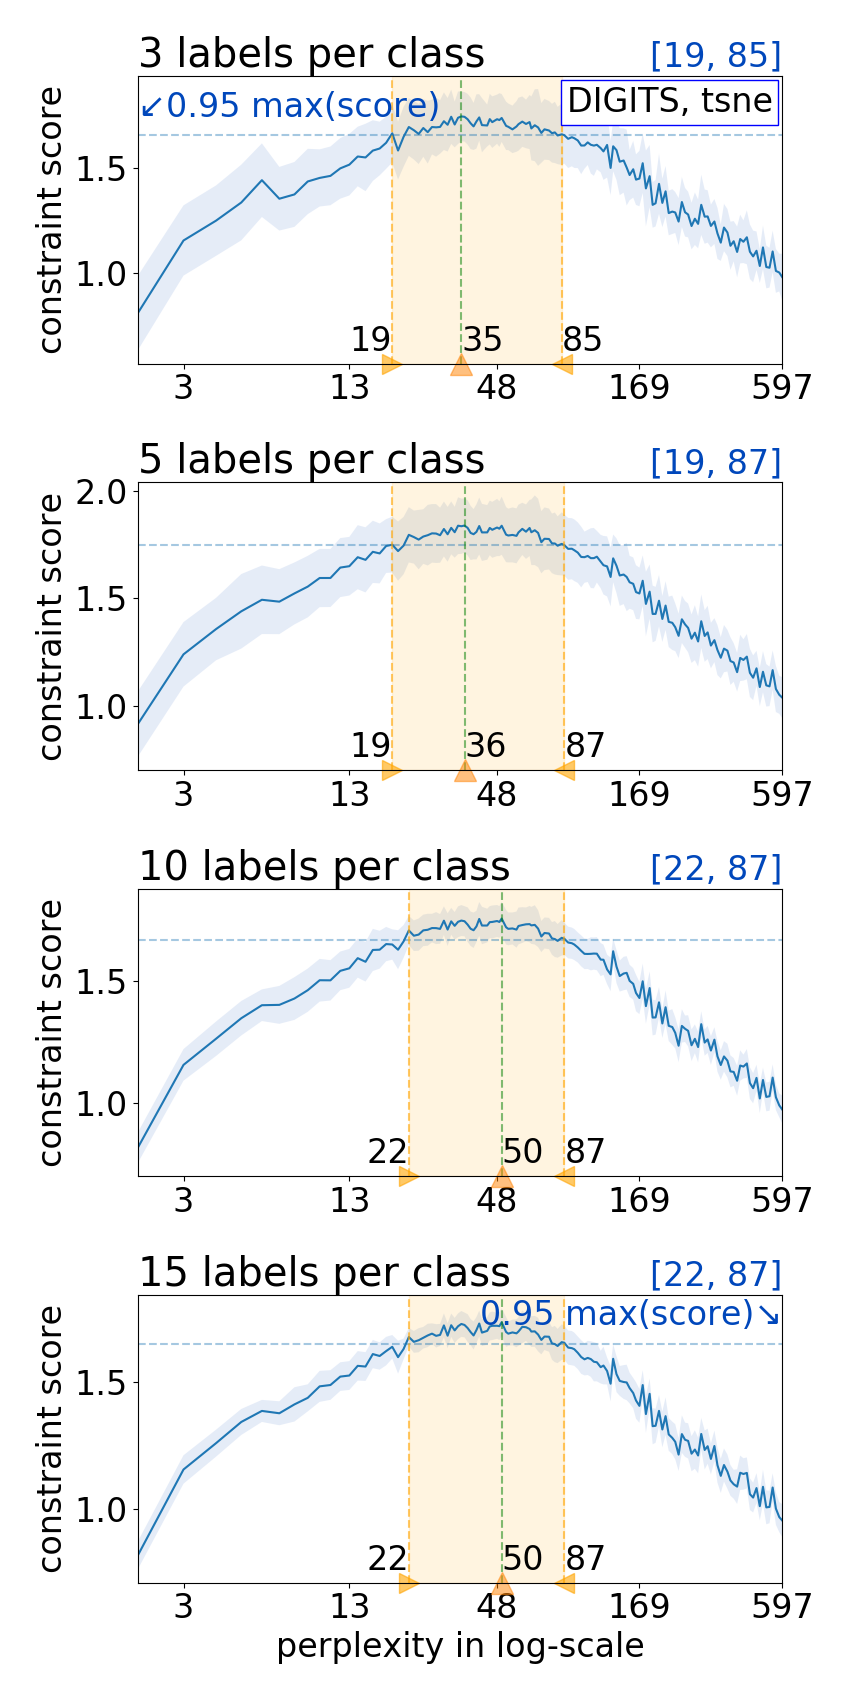
\includegraphics[width=\textwidth]{DIGITS_tsne_scores}
%         \caption{DIGITS}
%     \end{subfigure}
%     ~
%     \begin{subfigure}[b]{0.152\textwidth}
%         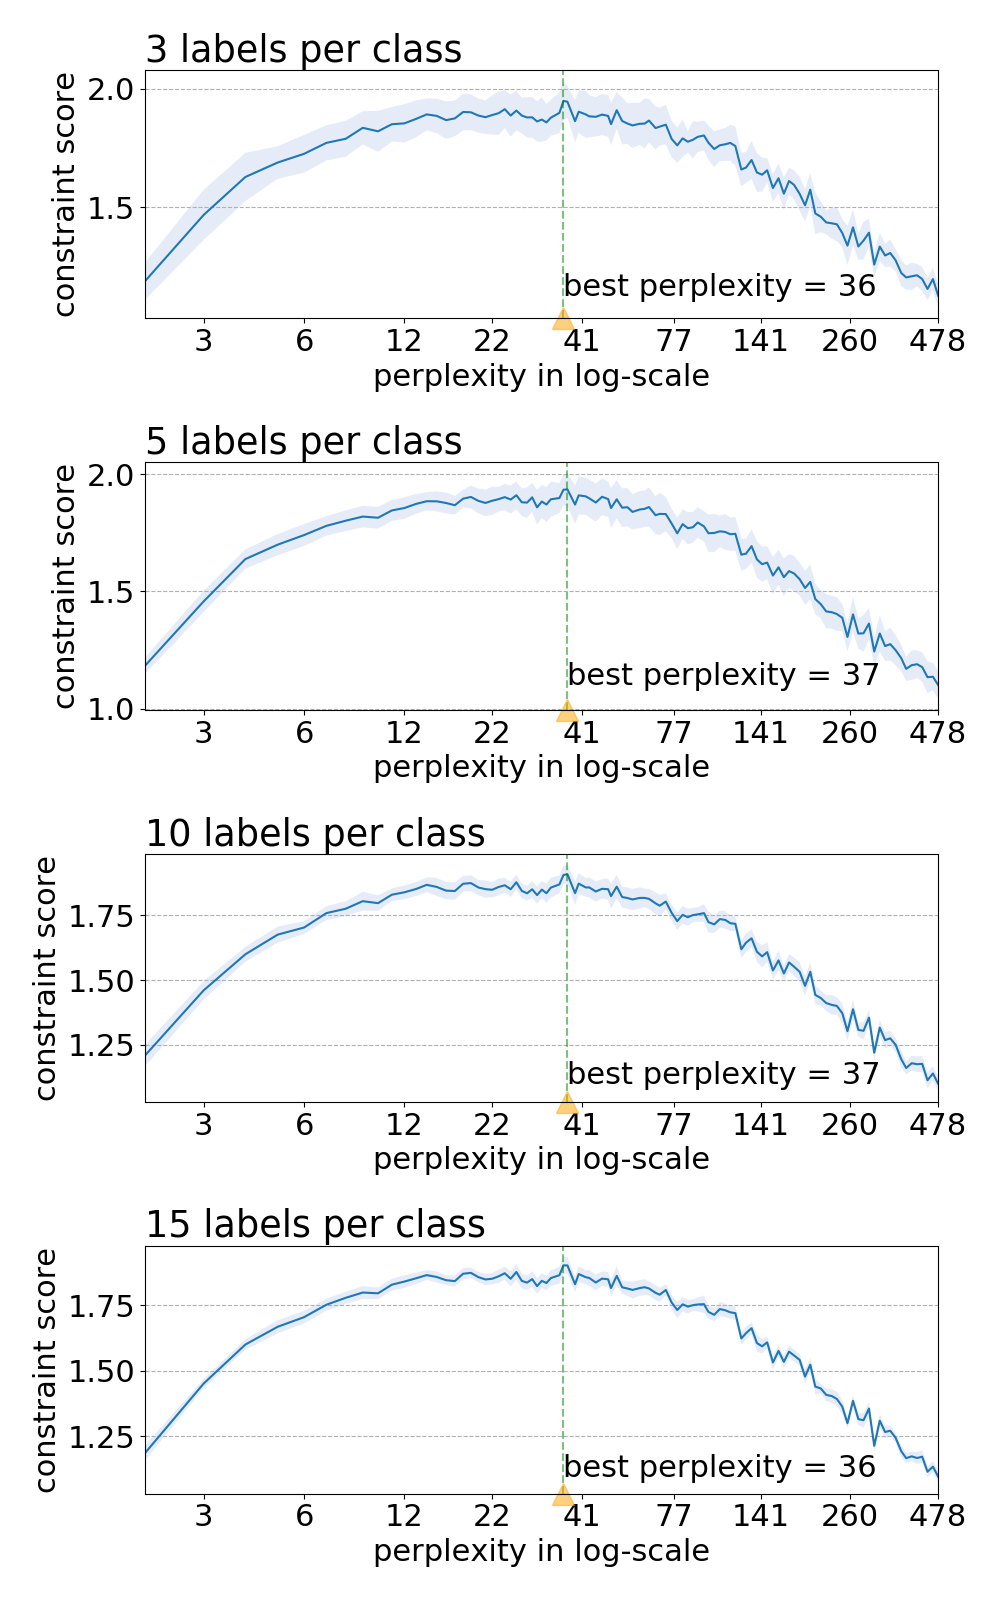
\includegraphics[width=\textwidth]{COIL20_tsne_scores}
%         \caption{COIL20}
%     \end{subfigure}
%     ~
%     \begin{subfigure}[b]{0.152\textwidth}
%         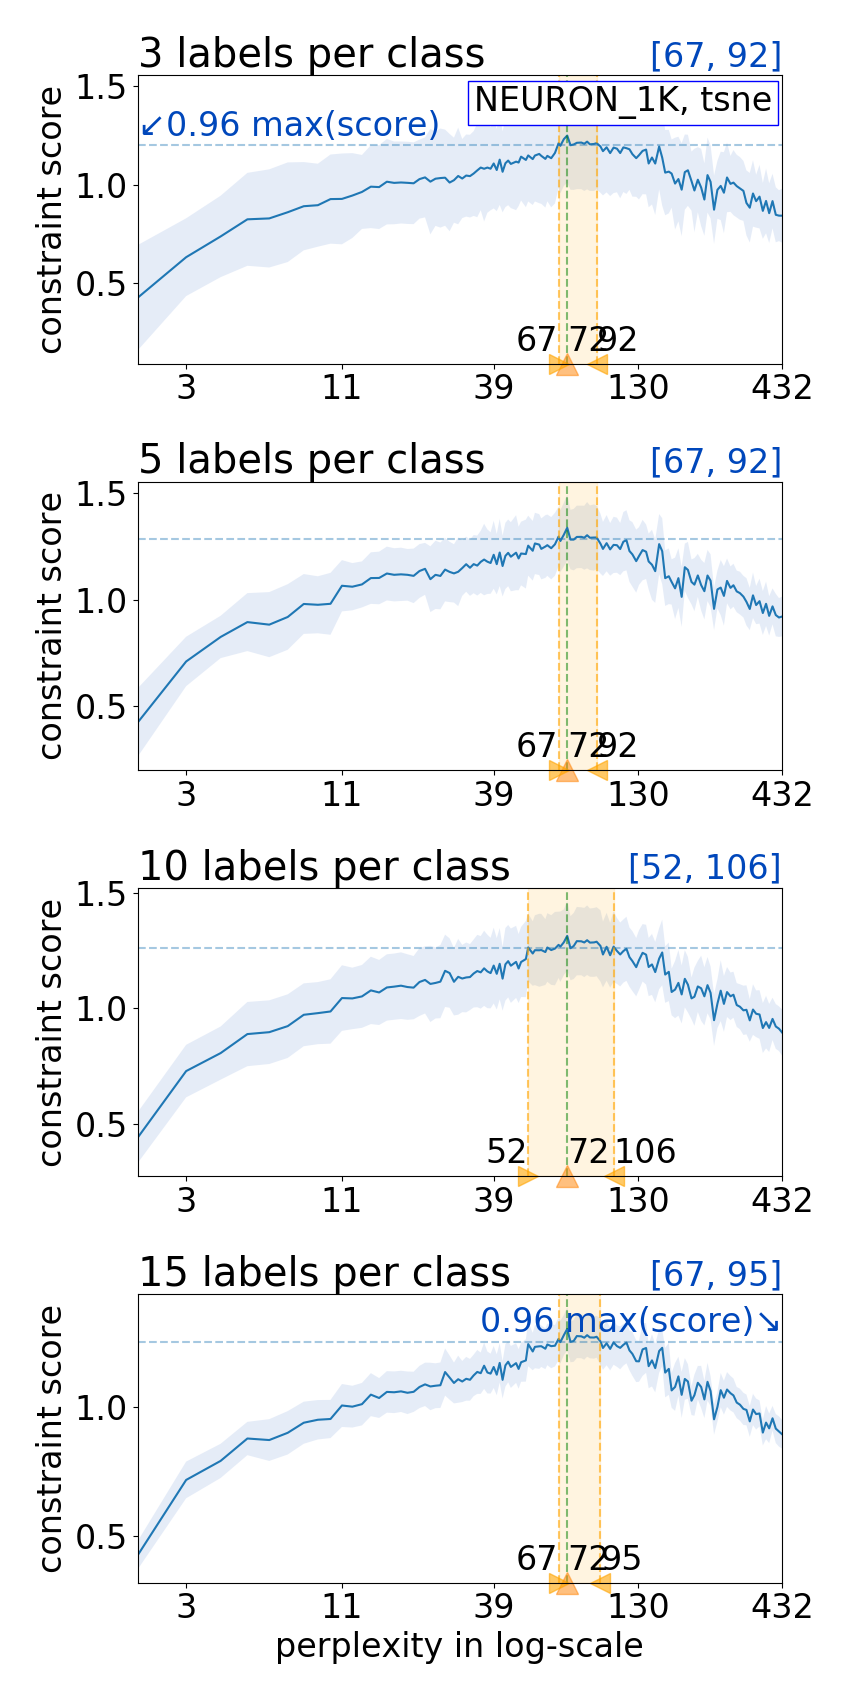
\includegraphics[width=\textwidth]{NEURON_1K_tsne_scores}
%         \caption{NEURON\_1K}
%     \end{subfigure}
%     ~
%     \begin{subfigure}[b]{0.152\textwidth}
%         \centering
%         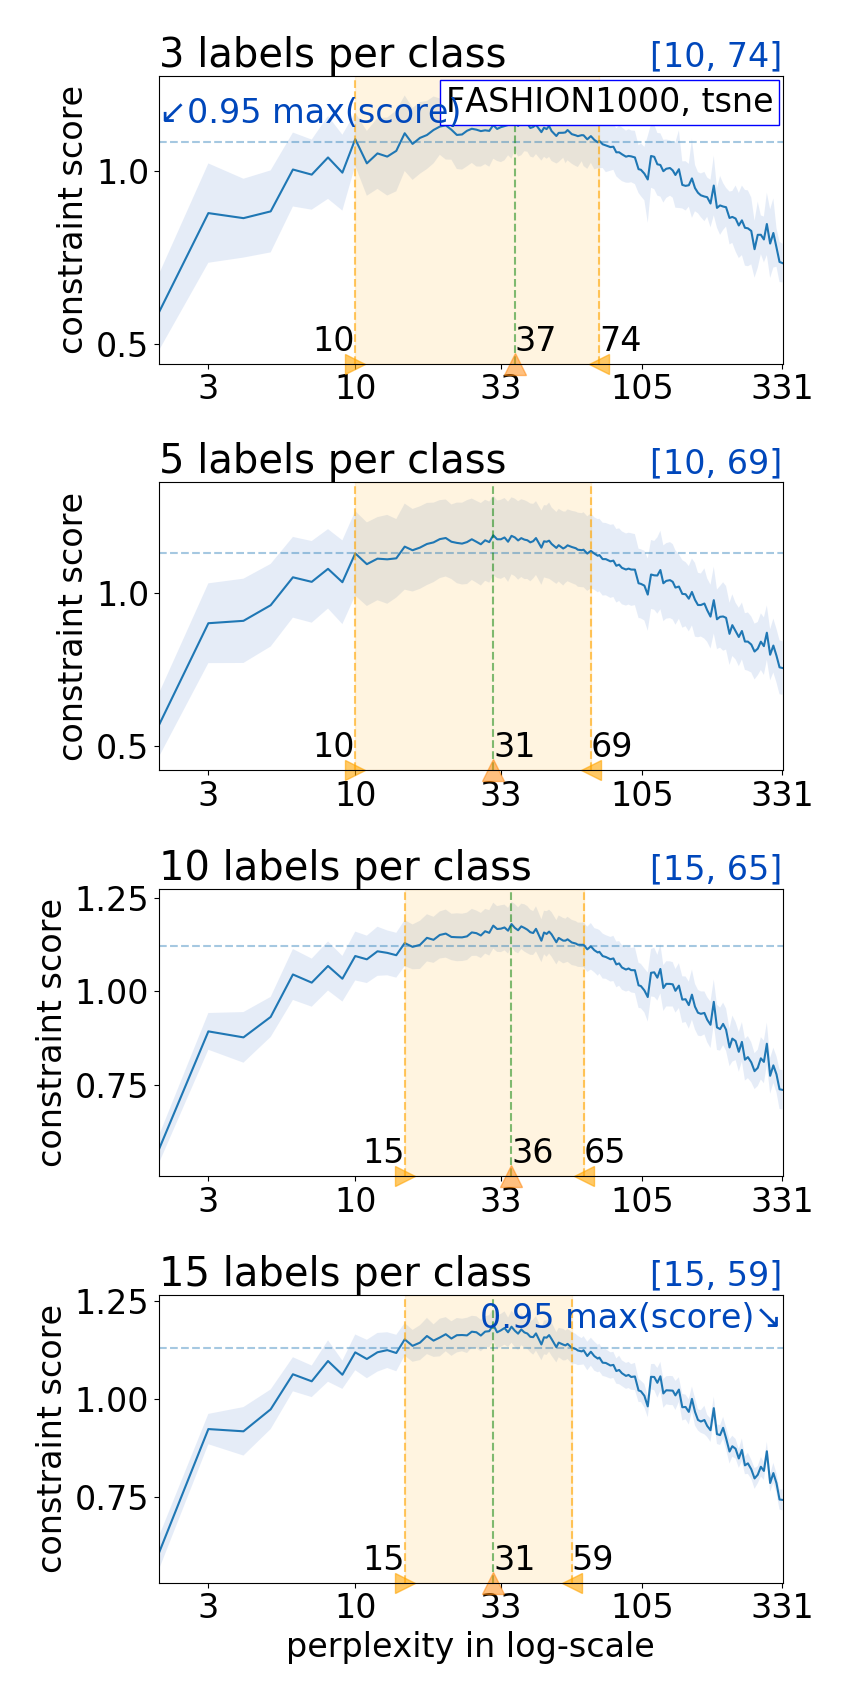
\includegraphics[width=\textwidth]{FASHION1000_tsne_scores}
%         \caption{FASHION1000}
%     \end{subfigure}
%     ~
%     \begin{subfigure}[b]{0.152\textwidth}
%         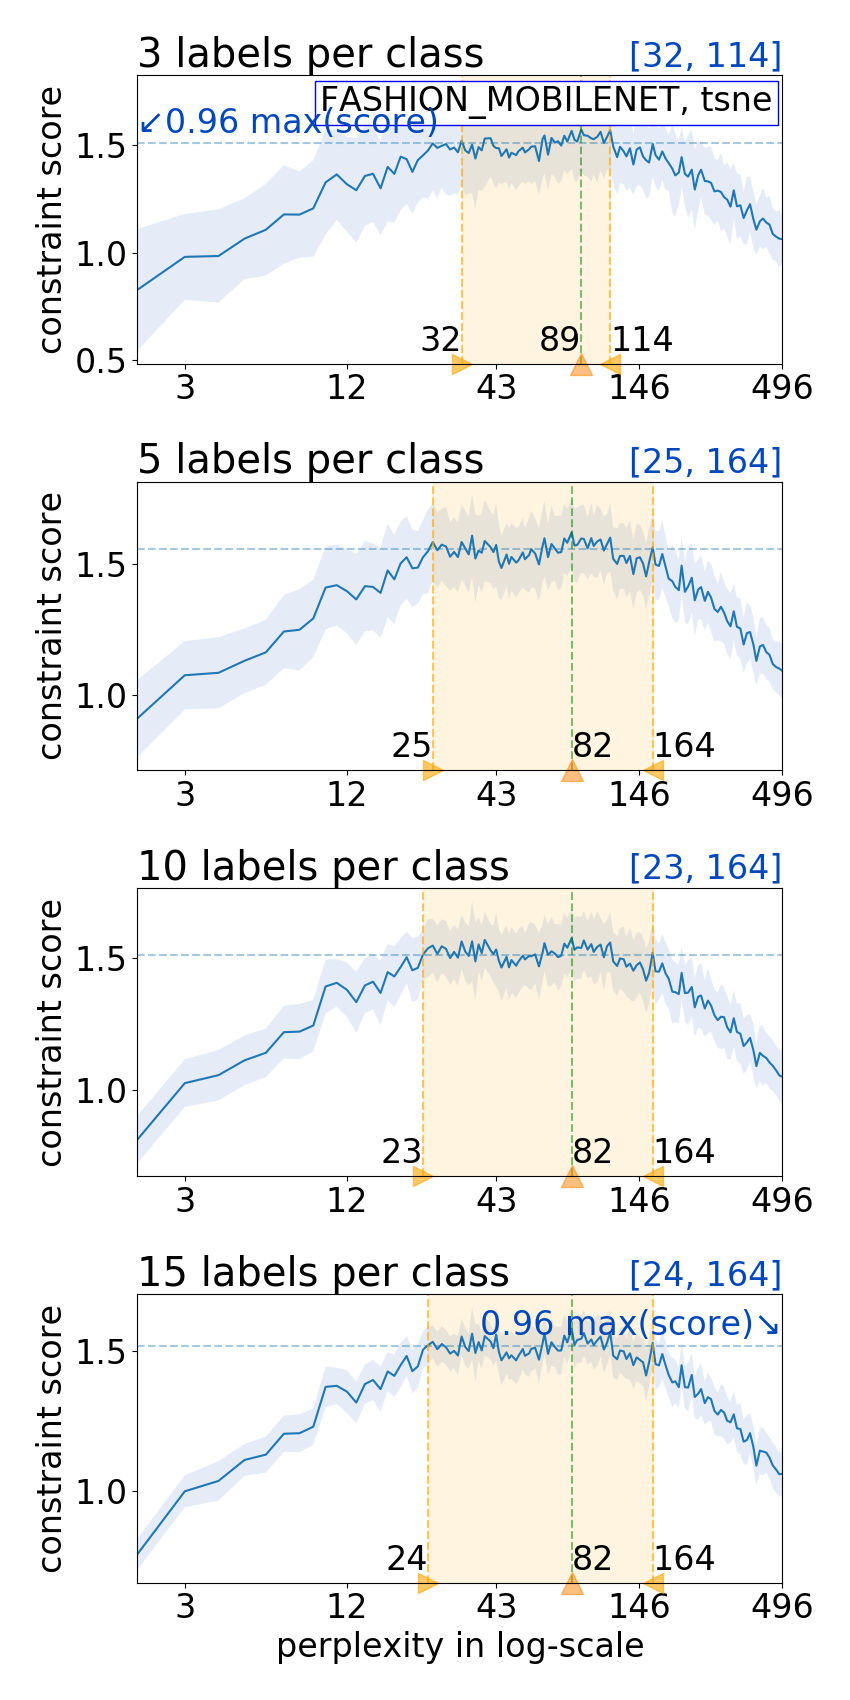
\includegraphics[width=\textwidth]{FASHION_MOBILENET_tsne_scores}
%         \caption{F\_MOBILENET}
%     \end{subfigure}
%     ~
%     \begin{subfigure}[b]{0.152\textwidth}
%         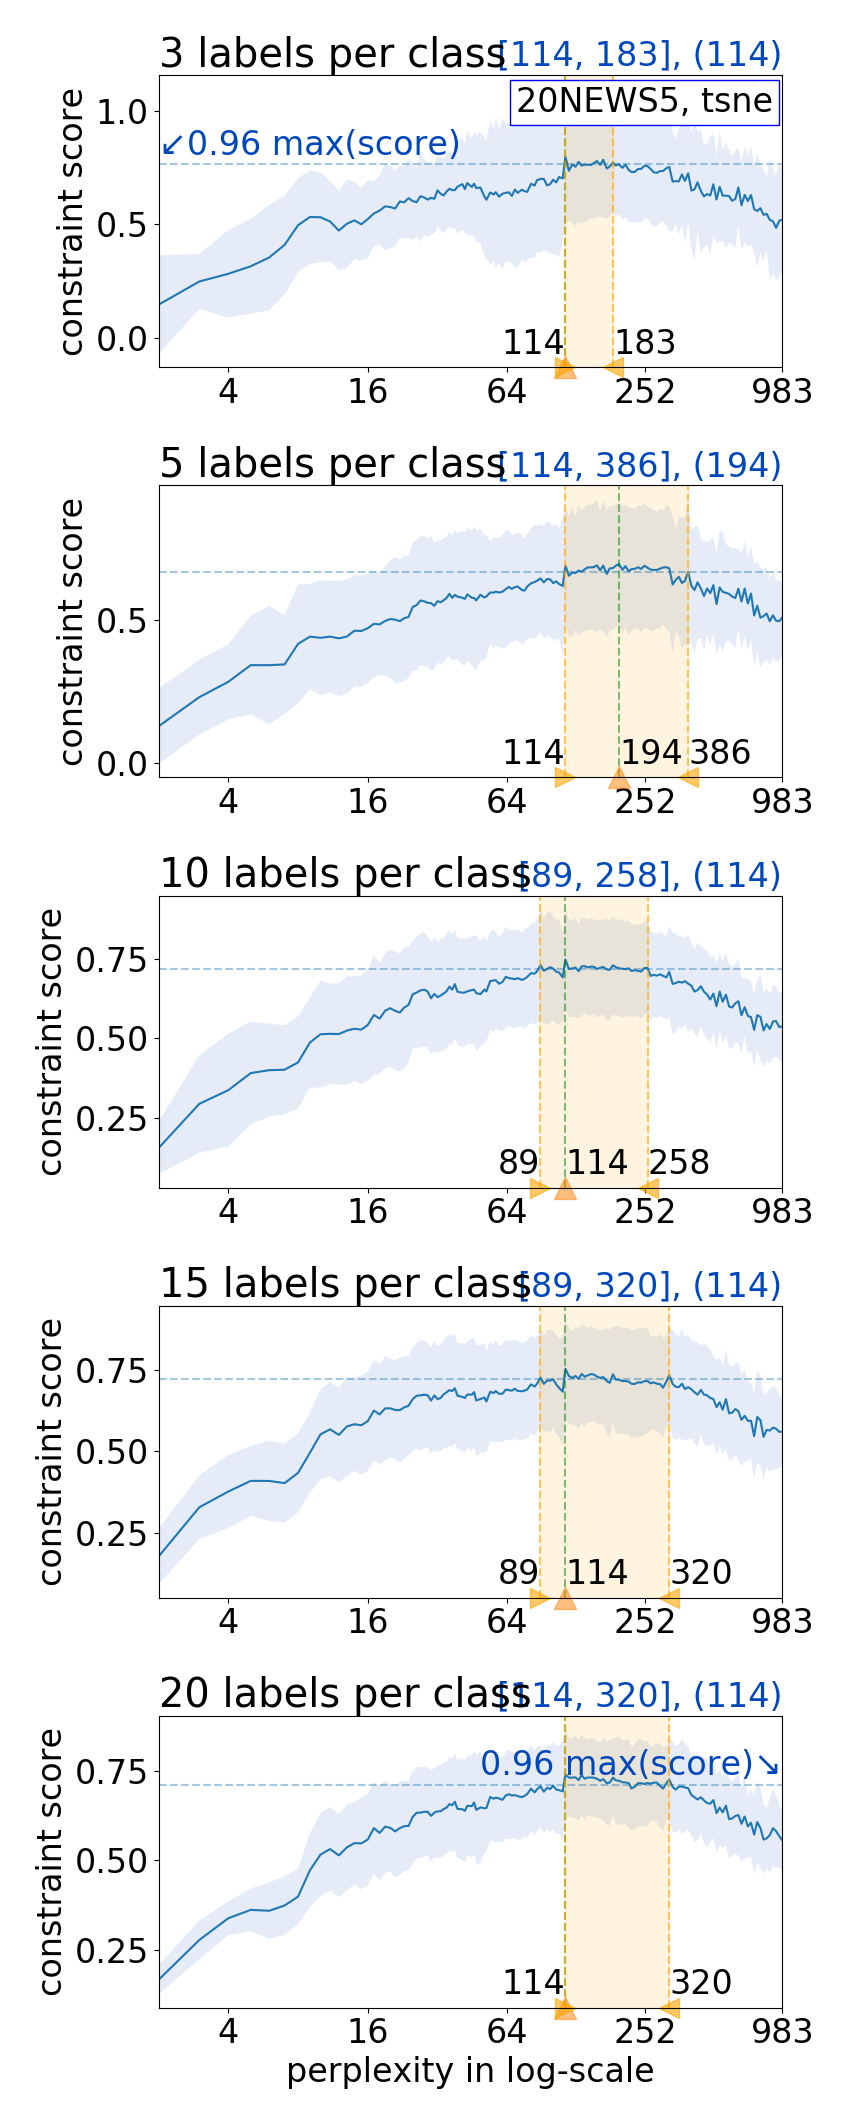
\includegraphics[width=\textwidth]{20NEWS5_tsne_scores}
%         \caption{20NEWS5}
%     \end{subfigure}
%     \caption{Stability of constraint preserving score with respect to different number of labeled instances for each class. The scores are calculated for all t-SNE embeddings.}
%     \label{fig:score:tsne:stability:annex}
% \end{figure*}


% \begin{figure*}%[pos=h]
%     \centering
%     \begin{subfigure}[b]{0.152\textwidth}
%         \centering
%         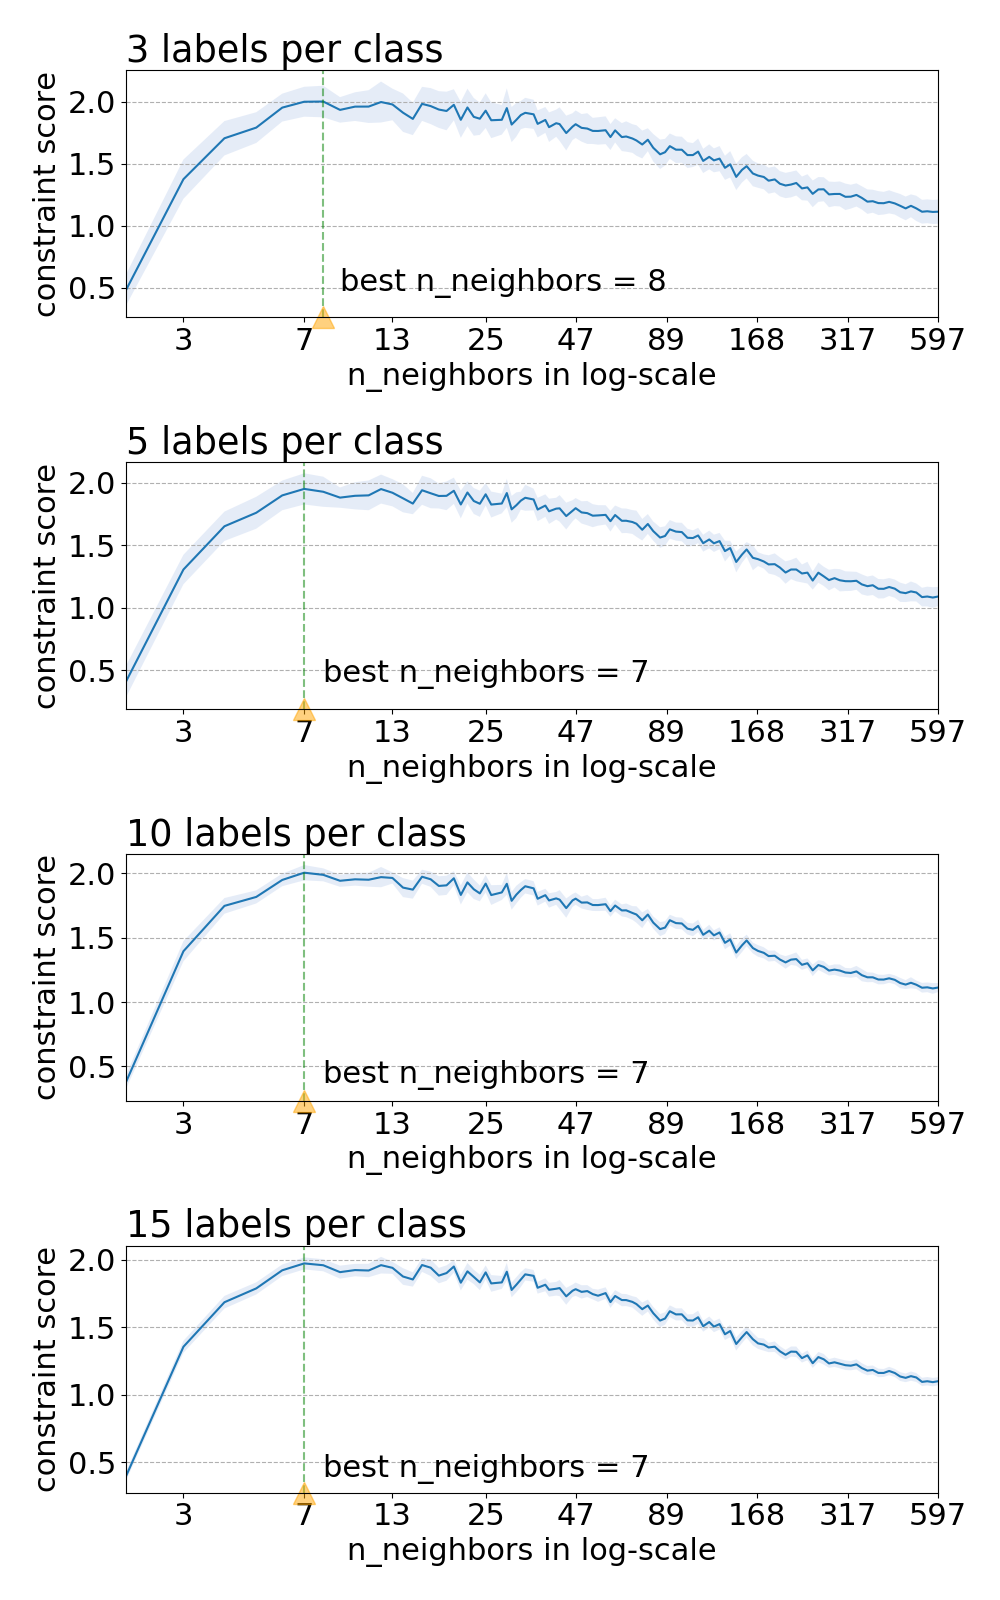
\includegraphics[width=\textwidth]{DIGITS_umap_scores}
%         \caption{DIGITS}
%     \end{subfigure}
%     ~
%     \begin{subfigure}[b]{0.152\textwidth}
%         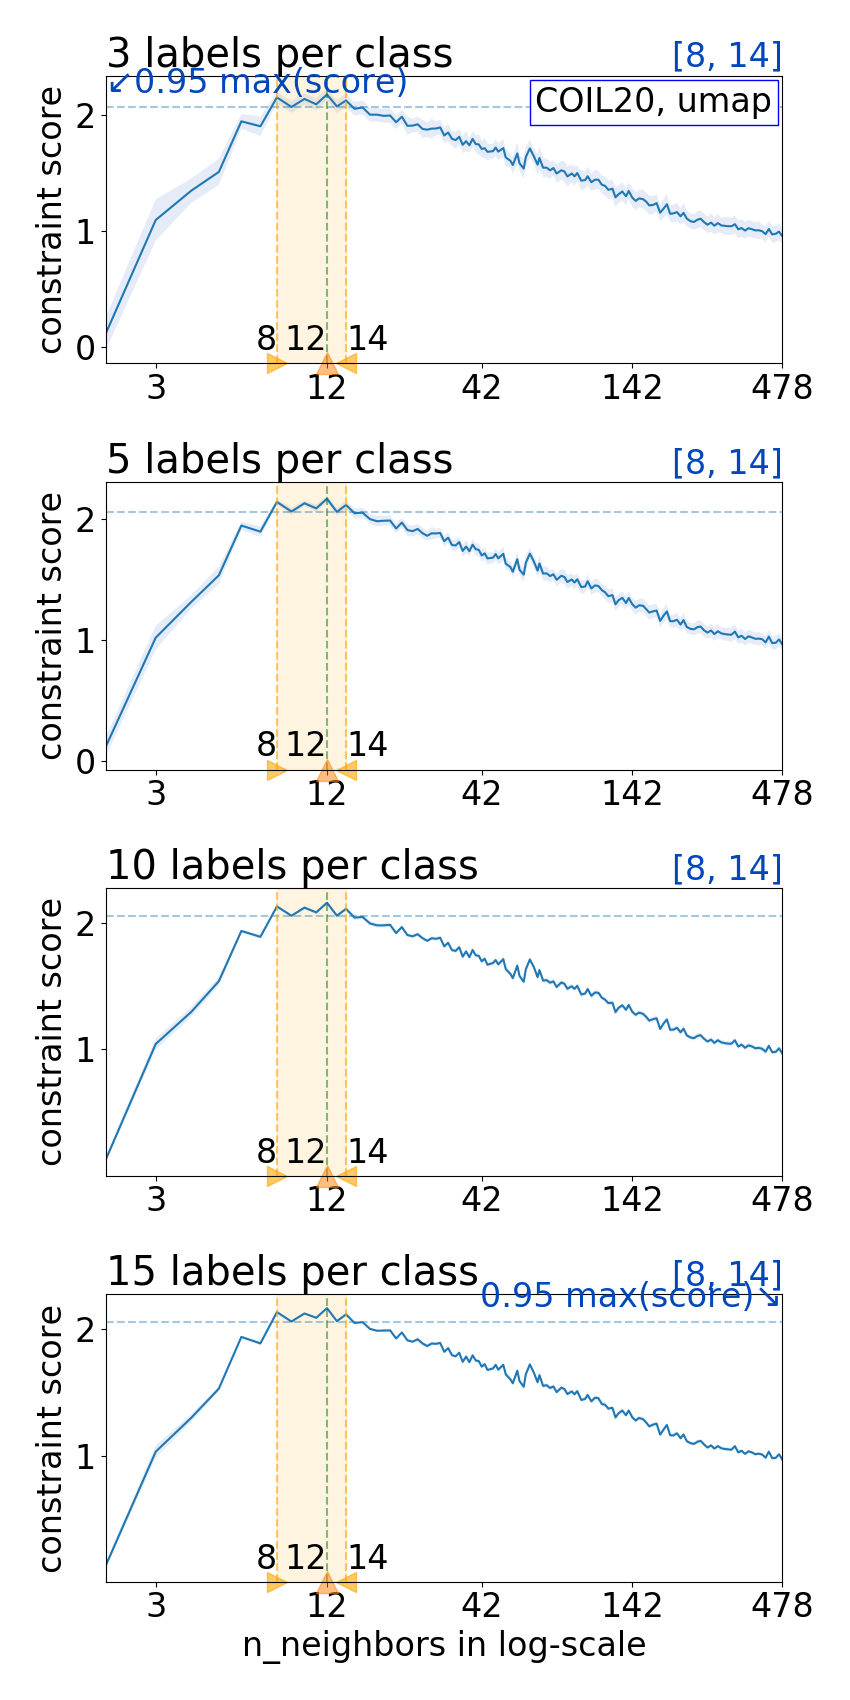
\includegraphics[width=\textwidth]{COIL20_umap_scores}
%         \caption{COIL20}
%     \end{subfigure}
%     ~
%     \begin{subfigure}[b]{0.152\textwidth}
%         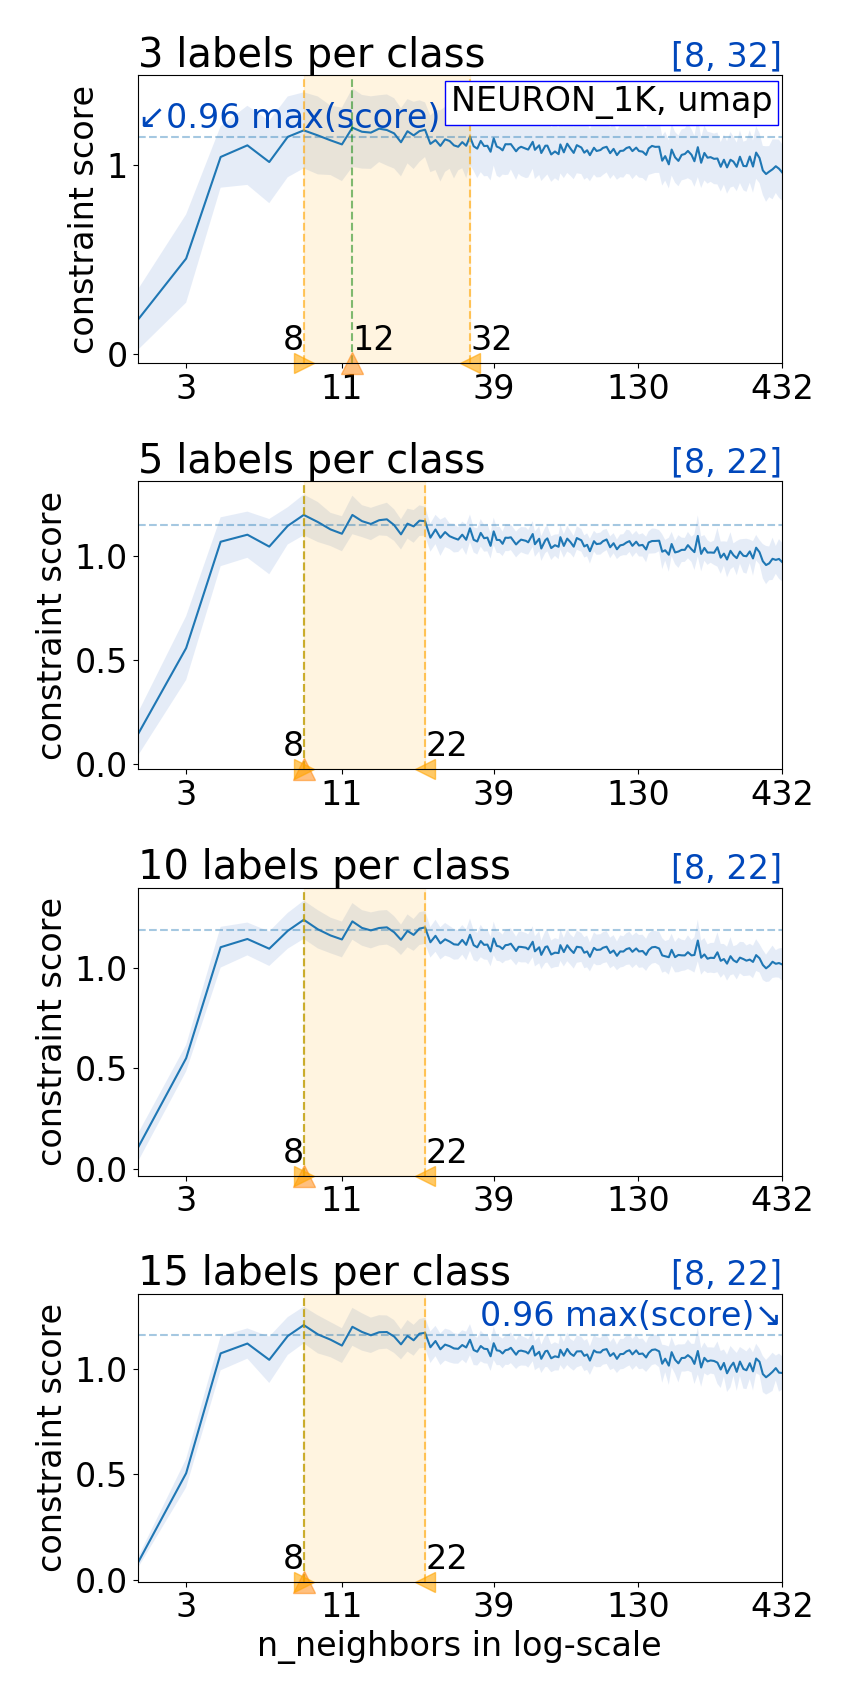
\includegraphics[width=\textwidth]{NEURON_1K_umap_scores}
%         \caption{NEURON\_1K}
%     \end{subfigure}
%     ~
%     \begin{subfigure}[b]{0.152\textwidth}
%         \centering
%         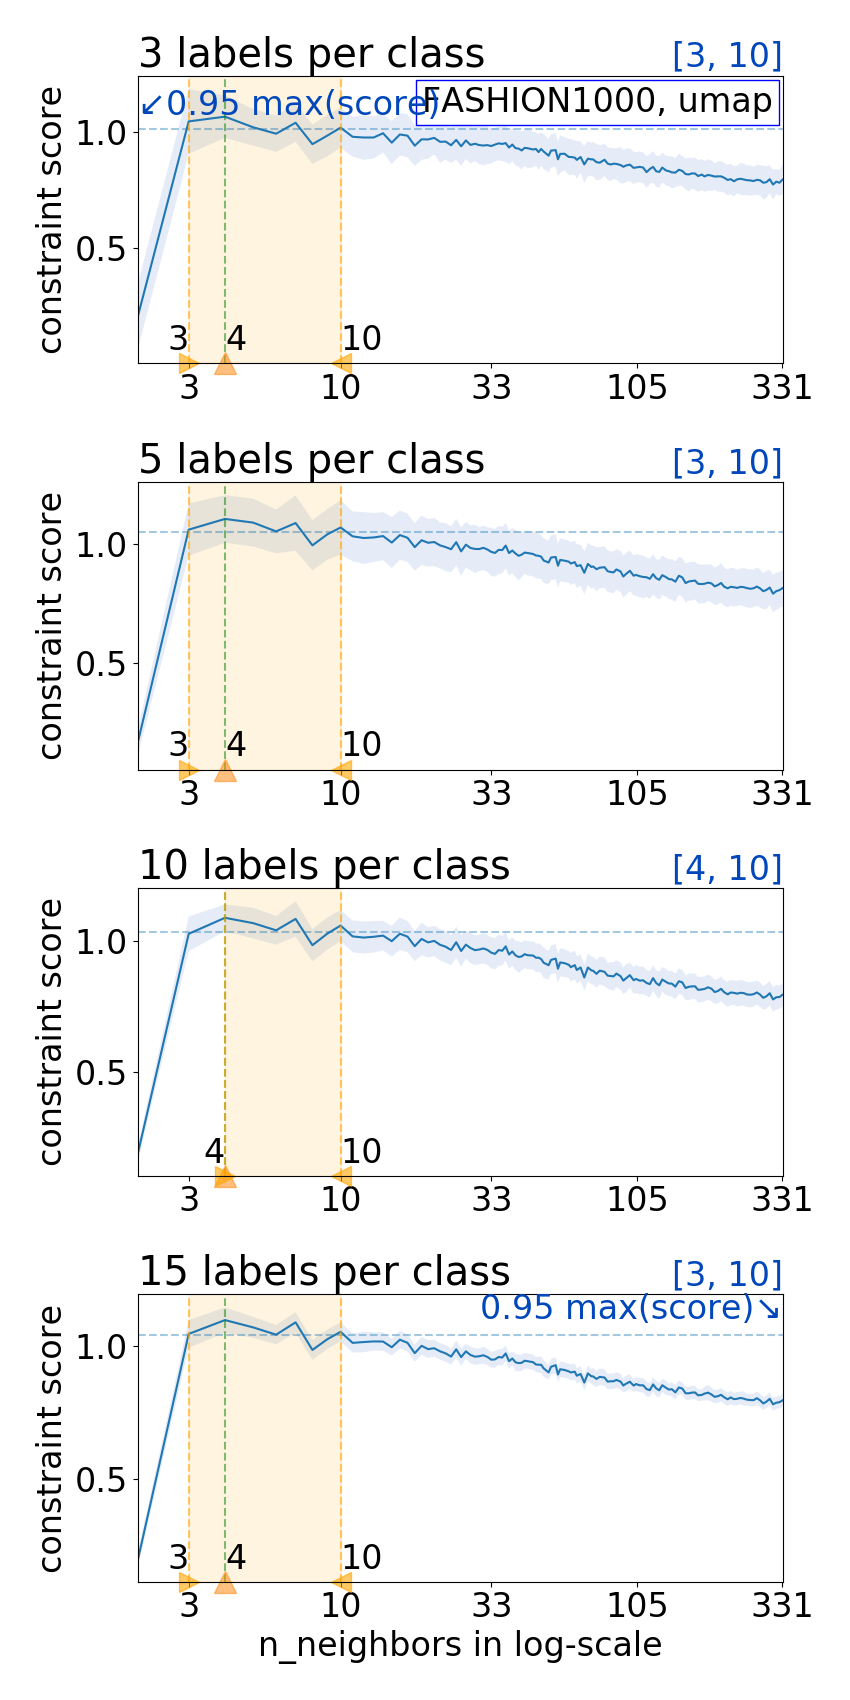
\includegraphics[width=\textwidth]{FASHION1000_umap_scores}
%         \caption{FASHION1000}
%     \end{subfigure}
%     ~
%     \begin{subfigure}[b]{0.152\textwidth}
%         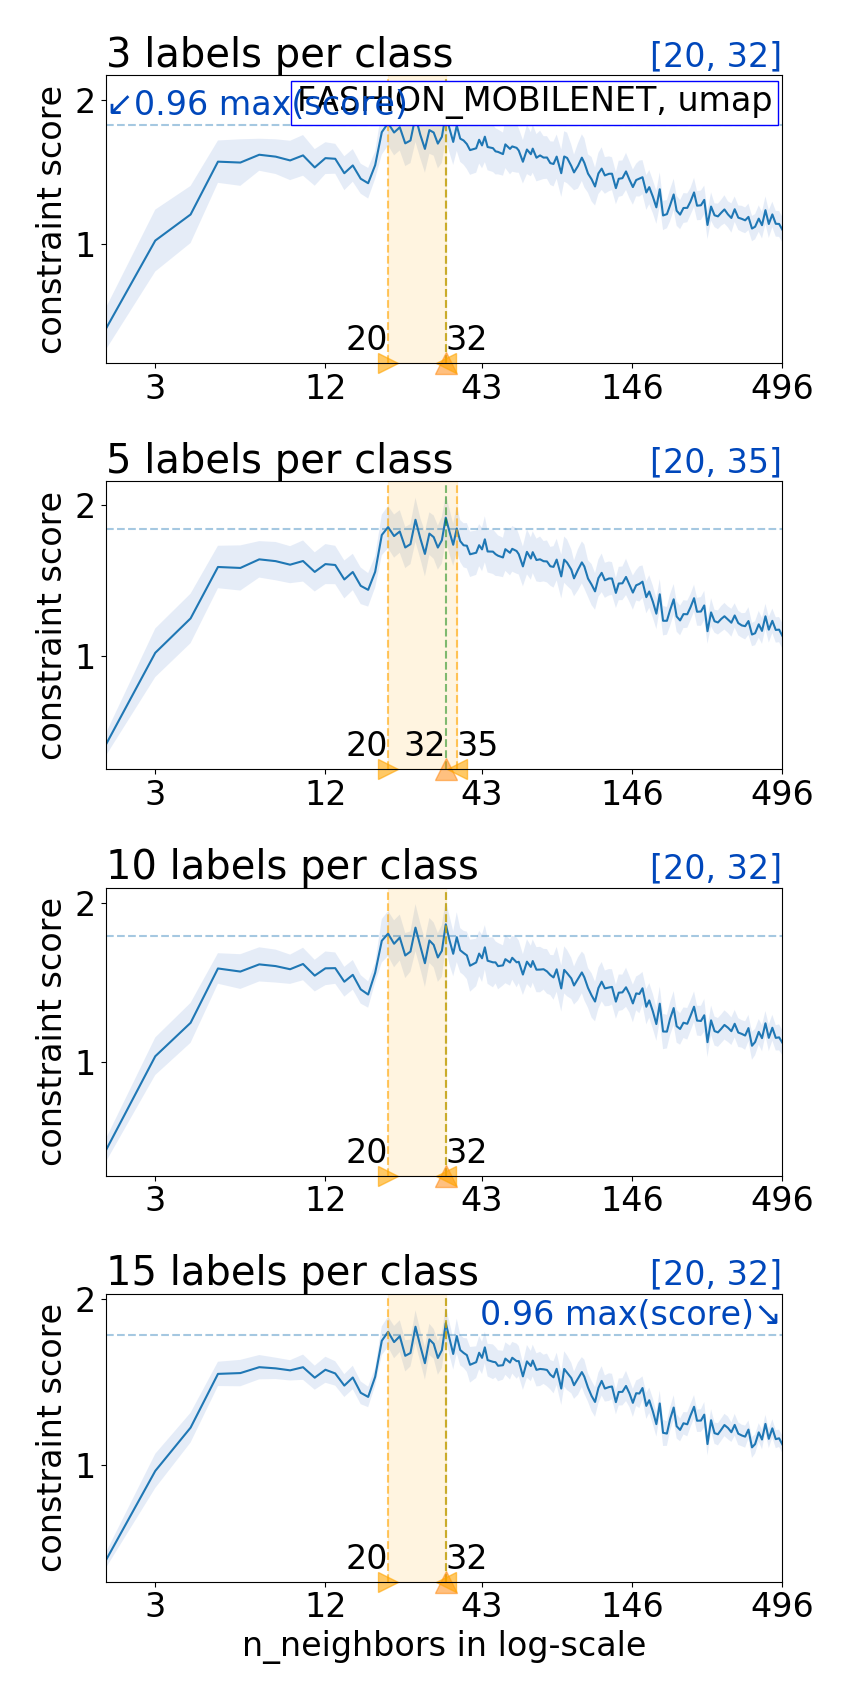
\includegraphics[width=\textwidth]{FASHION_MOBILENET_umap_scores}
%         \caption{F\_MOBILENET}
%     \end{subfigure}
%     ~
%     \begin{subfigure}[b]{0.152\textwidth}
%         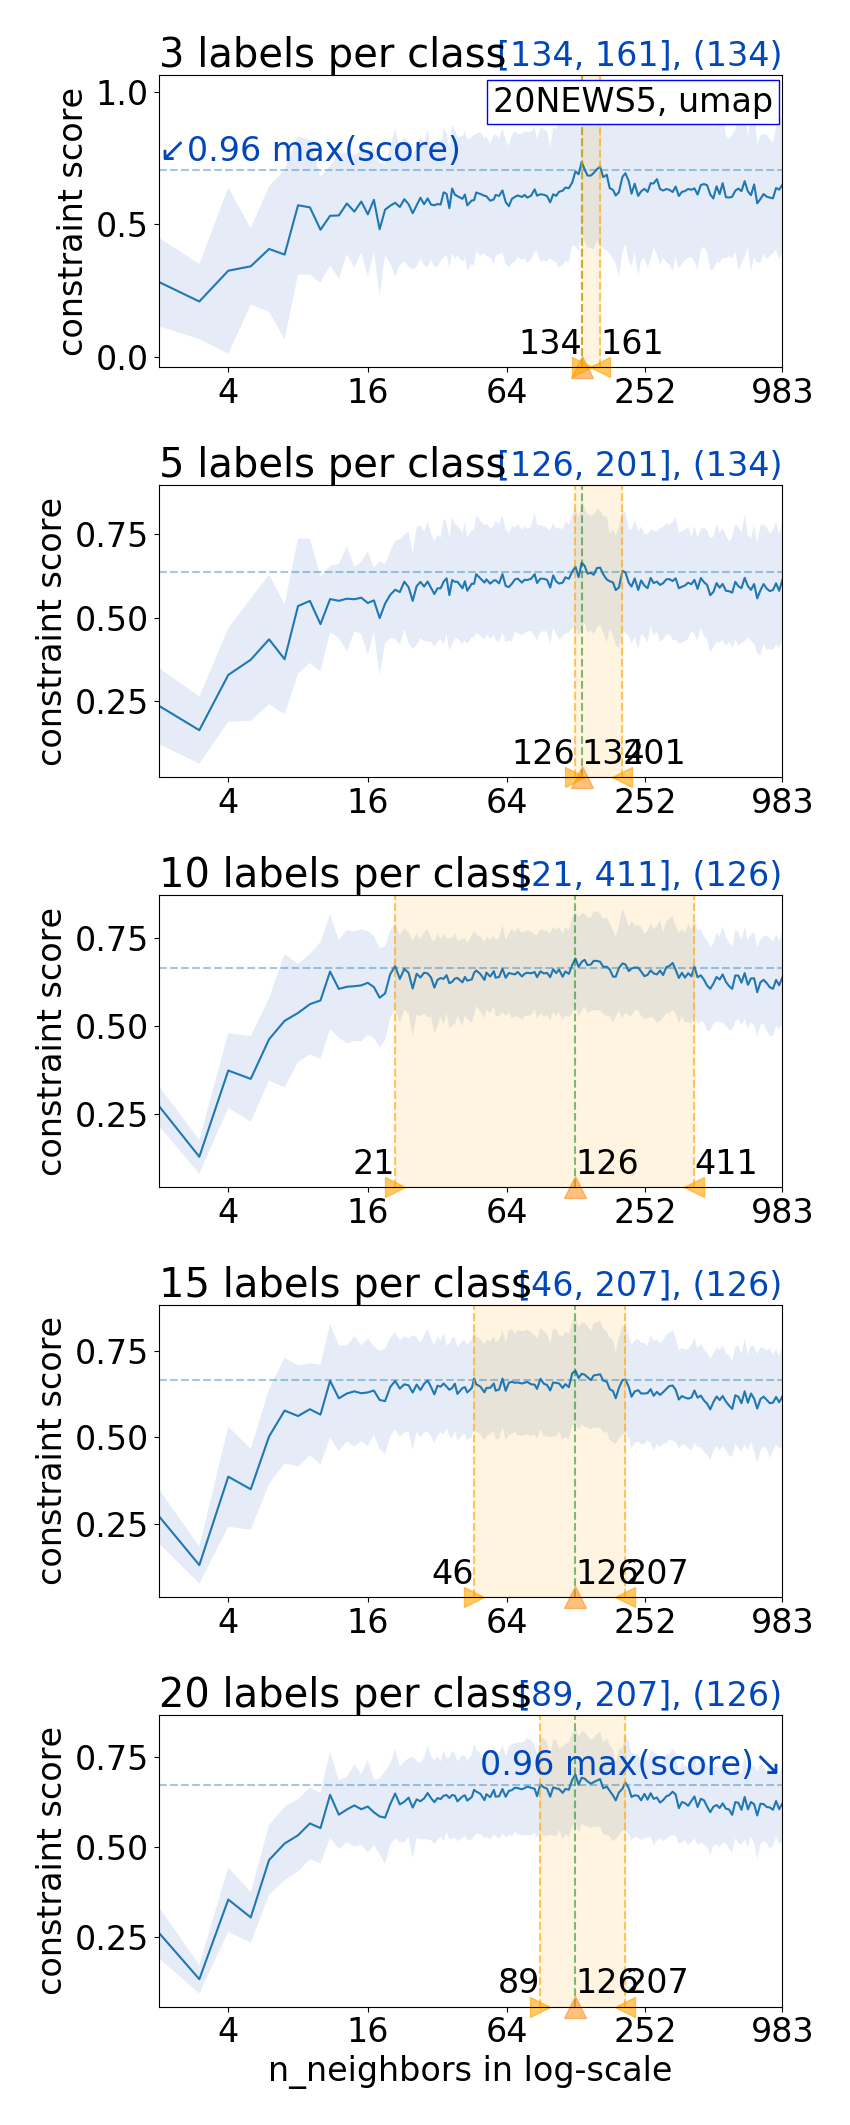
\includegraphics[width=\textwidth]{20NEWS5_umap_scores}
%         \caption{20NEWS5}
%     \end{subfigure}
%     \caption{Stability of constraint preserving score with respect to different number of labeled instances for each class. The scores are calculated for all UMAP embeddings with varied \emph{n\_neighbors} and fixed \emph{min\_dist} of 0.1.}
%     \label{fig:score:umap:stability:annex}
% \end{figure*}


% %%%%%%%%%%%%%%%%%%%%%%%%%%%%%%%%%%%%%%%%%%%%%%%%%%%%%%%%%%%%%%%%%%%%%%%%%%%%%%%%%%%%%%%%%%%%%%%
% \section{Metamap and samples for t-SNE's embeddings with \emph{DIGITS} and \emph{FASHION\_1K} datasets}\label{app:tsne:meta}

% \begin{figure*}%[pos=h]
%     \centering
%     \begin{subfigure}[b]{\textwidth}
%         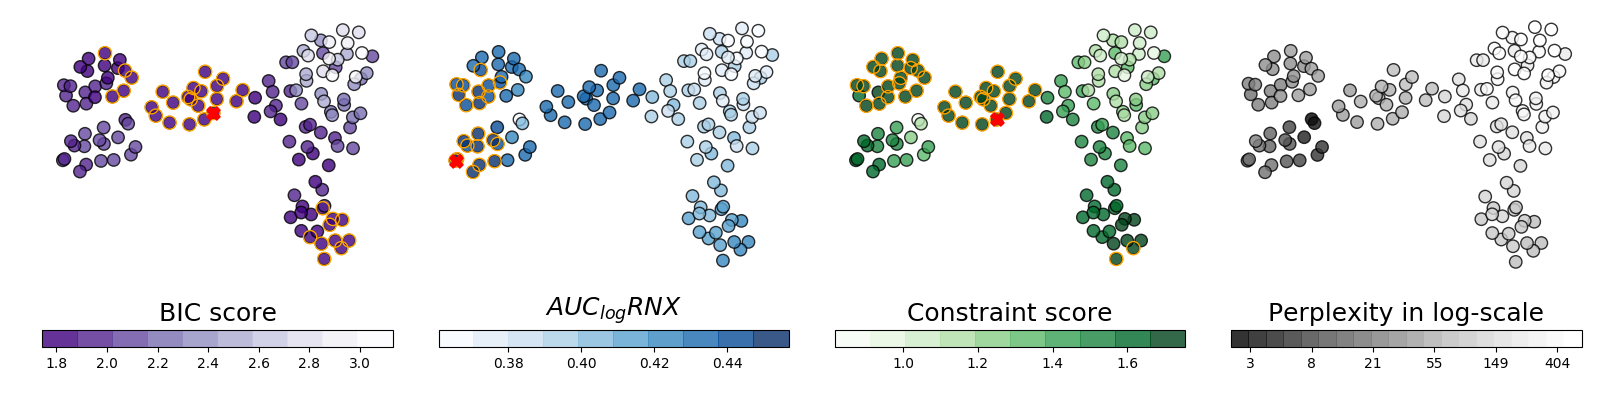
\includegraphics[width=\textwidth]{DIGITS_tsne_metamap}
%         \caption{Metamap and sample visualizations for the selected parameters for \emph{DIGITS} dataset.}
%     \label{fig:app:tsne:meta:DIGITS}
%     \end{subfigure}
%     ~
%     \begin{subfigure}[b]{\textwidth}
%         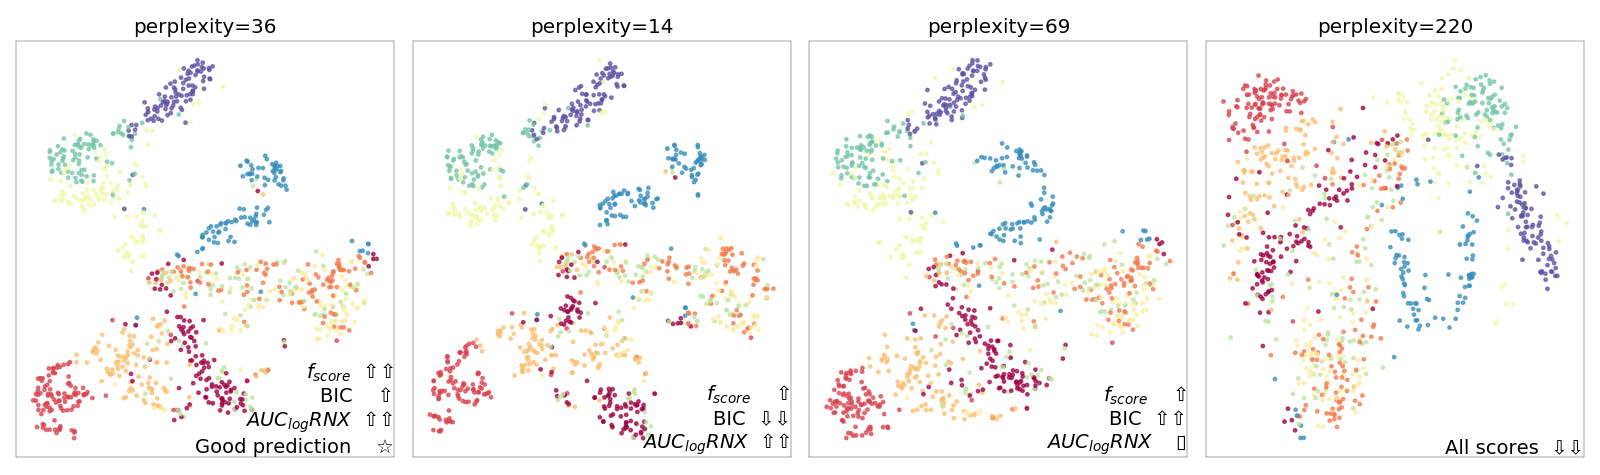
\includegraphics[width=\textwidth]{FASHION1000_tsne_show}
%         \caption{Metamap and sample visualizations for the selected parameters for \emph{FASHION\_1K} dataset.}
%     \label{fig:app:tsne:meta:FASHION1K}
%     \end{subfigure}
% \end{figure*}

% For the \emph{FASHION\_1K} dataset, the good perplexities found by $f_{score}$ agree with both $AUC_{log}RNX$ and BIC-based score.
% These score together discover the good region in the solution space (visualized by the metamap).
% The visualizations corresponding to the best perplexities found by three scores
% and an counter-intuitive example for the bad region in the solution space are shown for qualitative comparison.


% %%%%%%%%%%%%%%%%%%%%%%%%%%%%%%%%%%%%%%%%%%%%%%%%%%%%%%%%%%%%%%%%%%%%%%%%%%%%%%%%%%%%%%%%%%%%%%%
% \section{Compare $f_{score}$ with $AUC_{log}RNX$ (default min\_dist 0.1)}\label{app:score:umap:compare}
% See Fig.~\ref{fig:umap:compare}.

% \begin{figure*}%[pos=h]
%     \centering
%     \begin{subfigure}[b]{0.32\textwidth}
%         \centering
%         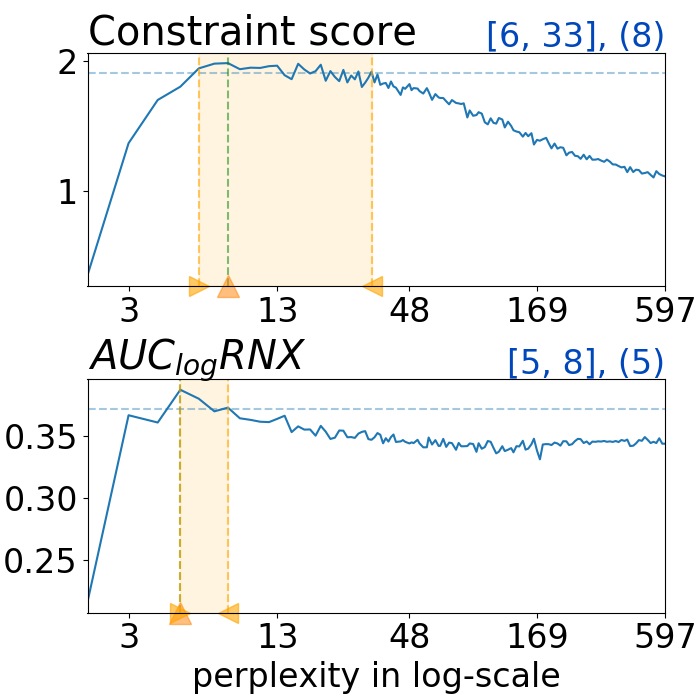
\includegraphics[width=\textwidth]{DIGITS_umap_compare_scores}
%         \caption{DIGITS}
%     \end{subfigure}
%     ~
%     \begin{subfigure}[b]{0.32\textwidth}
%         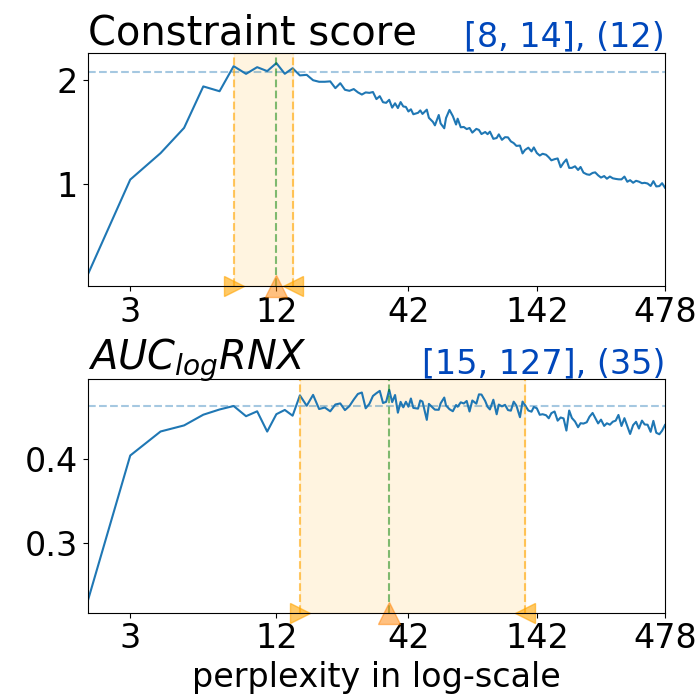
\includegraphics[width=\textwidth]{COIL20_umap_compare_scores}
%         \caption{COIL20}
%     \end{subfigure}
%     ~
%     \begin{subfigure}[b]{0.32\textwidth}
%         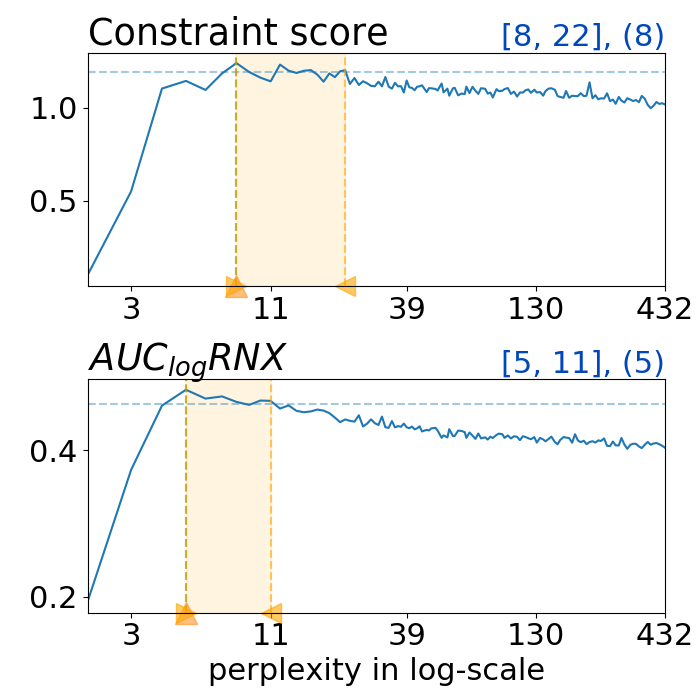
\includegraphics[width=\textwidth]{NEURON_1K_umap_compare_scores}
%         \caption{NEURON\_1K}
%     \end{subfigure}
%     \vfill
%     \begin{subfigure}[b]{0.32\textwidth}
%         \centering
%         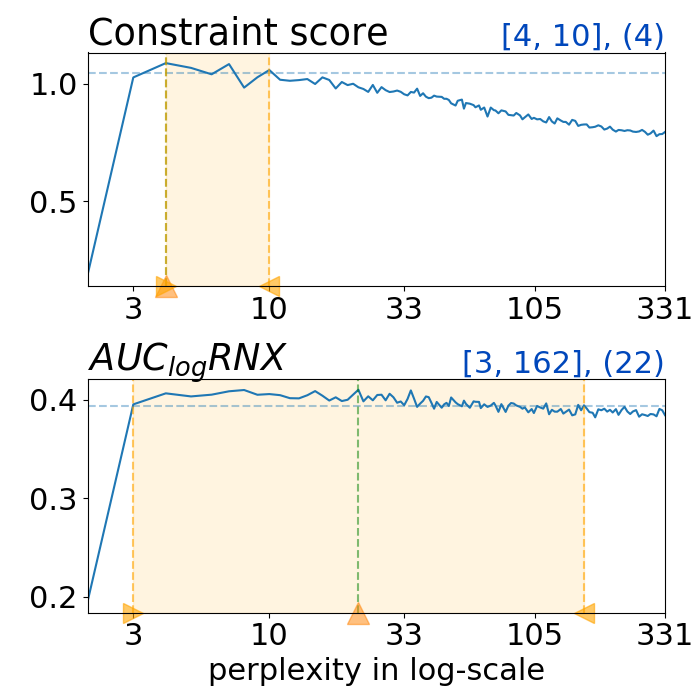
\includegraphics[width=\textwidth]{FASHION1000_umap_compare_scores}
%         \caption{FASHION1000}
%     \end{subfigure}
%     ~
%     \begin{subfigure}[b]{0.32\textwidth}
%         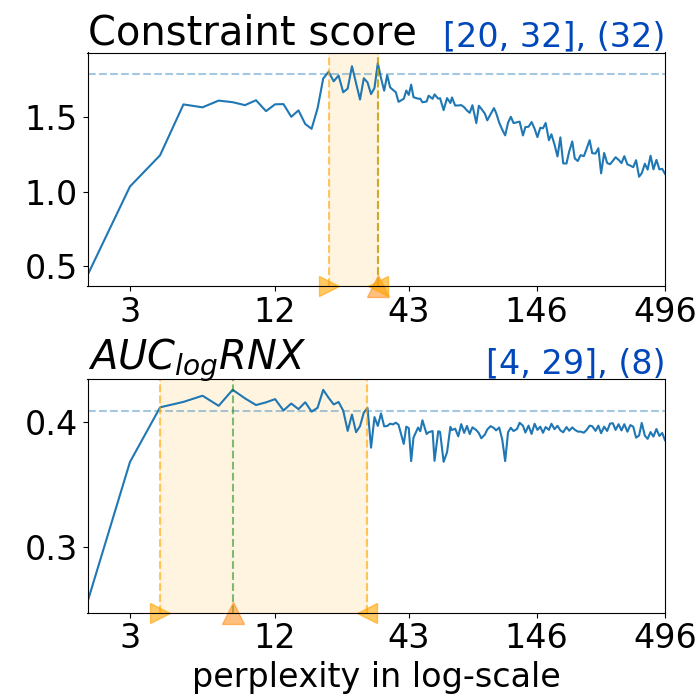
\includegraphics[width=\textwidth]{FASHION_MOBILENET_umap_compare_scores}
%         \caption{FASHION\_MOBILENET}
%     \end{subfigure}
%     ~
%     \begin{subfigure}[b]{0.32\textwidth}
%         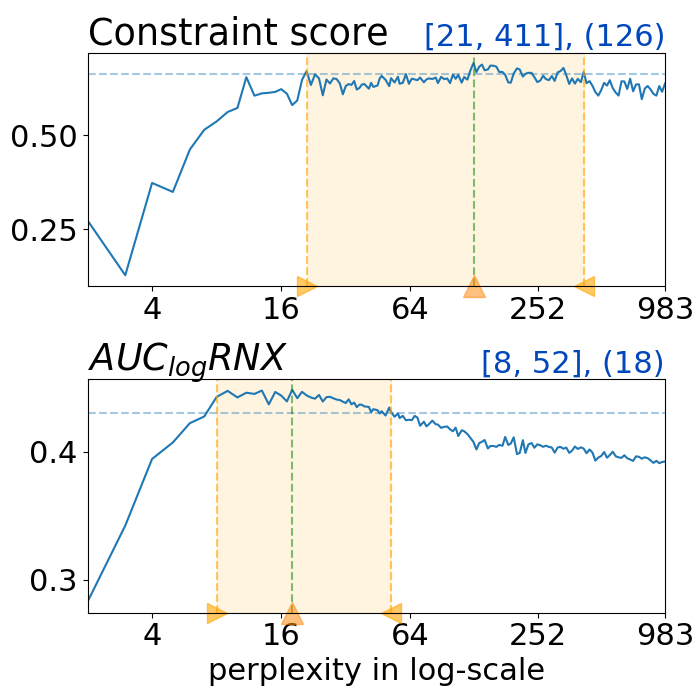
\includegraphics[width=\textwidth]{20NEWS5_umap_compare_scores}
%         \caption{20NEWS5}
%     \end{subfigure}
%     \caption{Comparing constraint score and $AUC_{log}RNX$ score for the embeddings of UMAP with fixed \texttt{min\_dist=0.1}.}
%     \label{fig:umap:compare}
% \end{figure*}


% \section{BayOpt for UMAP}
% BayOpt for UMAP with {FASHION\_1K} datasets\ref{fig:bo:umap:FASHION1K} and metatmap.

% \begin{figure}%[pos=h]
%     \begin{subfigure}[b]{.73\linewidth}
%         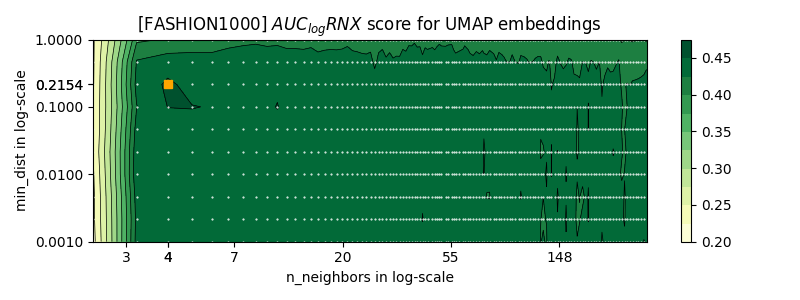
\includegraphics[width=\textwidth]{FASHION1000_umap_auc_rnx}
%         \caption{$AUC_{log}RNX$}
%     \end{subfigure}
%     ~
%     \begin{subfigure}[b]{.73\linewidth}
%         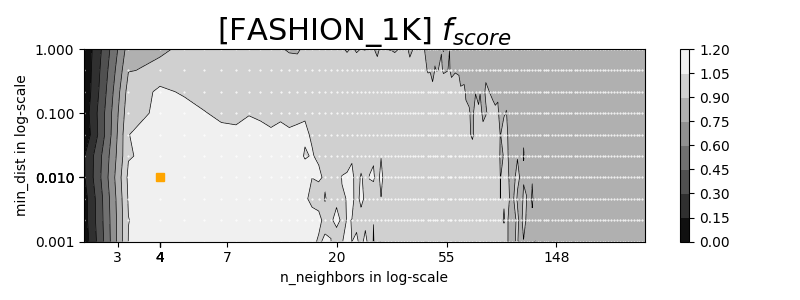
\includegraphics[width=\textwidth]{FASHION1000_umap_qij_score}
%         \caption{constraint score}
%     \end{subfigure}
%     ~
%     \begin{subfigure}[b]{\linewidth}
%         \centering
%         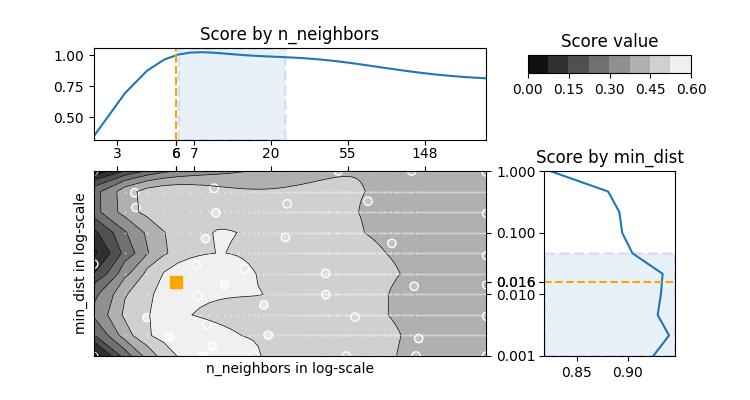
\includegraphics[width=\textwidth]{FASHION1000_umap_predicted_score}
%         \caption{BO predicted score}
%     \end{subfigure}
%     ~
%     \caption{\emph{FASHION\_1K}}
%     \label{fig:bo:umap:FASHION1K}
% \end{figure}

% \begin{figure*}
%     \centering
%     \begin{subfigure}[b]{\textwidth}
%         \centering
%         \includegraphics[width=\textwidth]{{FASHION1000_umap_metamap}.png}
%         \caption{Metamap for UMAP embeddings of FASHION1000 dataset.}
%     \end{subfigure}
%     ~
%     \begin{subfigure}[b]{\textwidth}
%         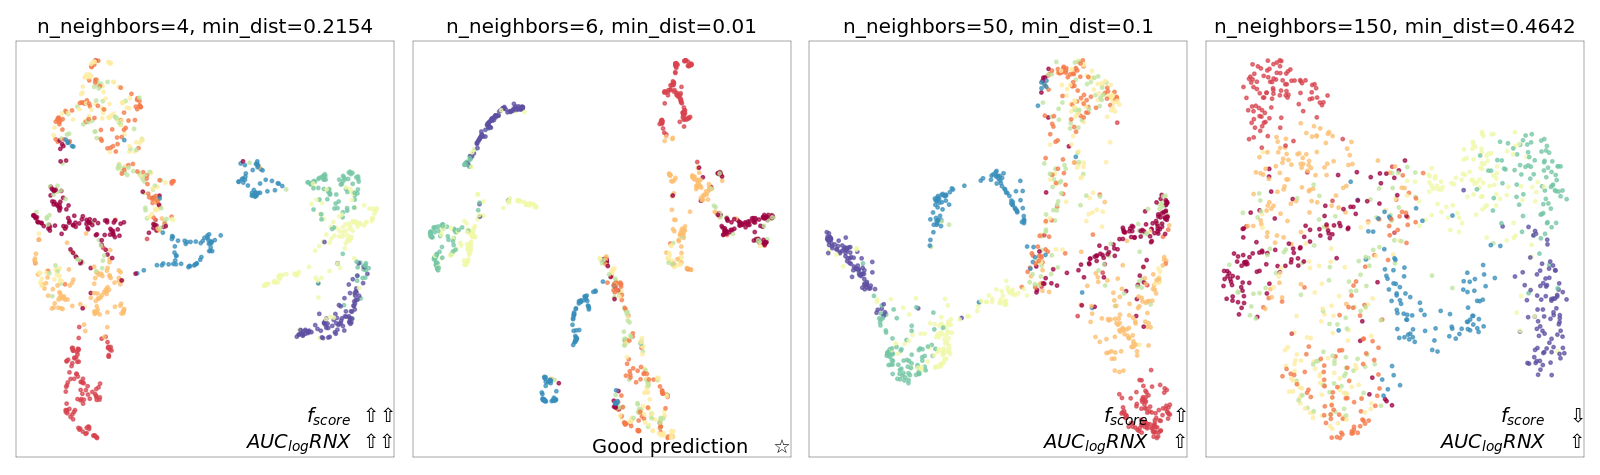
\includegraphics[width=\textwidth]{FASHION1000_umap_show}
%         \caption{Sample vizs FASHION1000}
%     \end{subfigure}
% \end{figure*}


% %%%%%%%%%%%%%%%%%%%%%%%%%%%%%%%%%%%%%%%%%%%%%%%%%%%%%%%%%%%%%%%%%%%%%%%%%%%%%%%%%%%%%%%%%%%%%%
% \section{Constraint-based Score as Target Function in Bayesian Optimization Approach}\label{app:bo:explain}

% + Explain the internal step in BayOpt.
% Can make use some figures Fig.~\ref{fig:bayopt5}, Fig.\ref{fig:bayopt10}.

% \begin{figure}
% \centering
% \includegraphics[scale=0.25]{{ucb_kappa5_constraint1.0_DIGITS_step5}.png}
% \caption{BayOpt after 5 steps.}\label{fig:bayopt5}
% \end{figure}


% \begin{figure}
% \centering
% \includegraphics[scale=0.25]{{ucb_kappa5_constraint1.0_DIGITS_step10}.png}
% \caption{BayOpt after 10 steps.}\label{fig:bayopt10}
% \end{figure}

% + Explain how the utility function are constructed and optimized, and answer why optimize the utility function (surrogate function), we can optimize at the same time the target function (the constraint-based score function).

% + Explain the exploitation-exploration trade-off in BayOpt (and estimate the number of times we need to try before reaching to the global maximum).

% %+ Note about the nature of BayOpt that, it can work with any non-convex multi-modal objective function and it assures to find the global extremum.